\documentclass[11pt,a4paper]{report}

\usepackage[utf8]{inputenc}
\usepackage[margin=0.8in]{geometry}
\usepackage{hyperref}
\usepackage{amsmath,amssymb}
\usepackage{listings}
\usepackage{xcolor}
\usepackage{graphicx}
\usepackage{tabularx}
\usepackage{booktabs}
\usepackage{fancyhdr}
\usepackage{titlesec}
\usepackage{enumitem}
\usepackage{microtype}
\usepackage[most]{tcolorbox}
\tcbuselibrary{listings, skins, breakable}
\usepackage{tikz}
\usetikzlibrary{shapes.geometric, arrows.meta, positioning, fit, calc, backgrounds, shadows}

% -------------------------------------------------------------------------
% COLOR PALETTE
% -------------------------------------------------------------------------
\definecolor{primaryblue}{rgb}{0.08, 0.38, 0.74}
\definecolor{darknavy}{rgb}{0.05, 0.15, 0.3}
\definecolor{accentteal}{rgb}{0.0, 0.55, 0.55}
\definecolor{codegreen}{rgb}{0.0, 0.5, 0.0}
\definecolor{codegray}{rgb}{0.45, 0.45, 0.45}
\definecolor{codepurple}{rgb}{0.55, 0.0, 0.65}
\definecolor{codebackground}{rgb}{0.97, 0.97, 0.98}
\definecolor{boxborder}{rgb}{0.8, 0.85, 0.92}

% -------------------------------------------------------------------------
% HYPERLINK CONFIGURATION
% -------------------------------------------------------------------------
\hypersetup{
    colorlinks=true,
    linkcolor=primaryblue,
    citecolor=primaryblue,
    urlcolor=primaryblue,
    pdftitle={Persona - Linkedin Scrapper platform: Complete Technical Reference Manual},
    pdfauthor={Team Persona}
}

% -------------------------------------------------------------------------
% LISTINGS STYLING
% -------------------------------------------------------------------------
\lstdefinestyle{customcode}{
    backgroundcolor=\color{codebackground},   
    commentstyle=\color{codegreen}\itshape,
    keywordstyle=\color{primaryblue}\bfseries,
    numberstyle=\tiny\color{codegray},
    stringstyle=\color{codepurple},
    basicstyle=\ttfamily\footnotesize,
    breakatwhitespace=false,         
    breaklines=true,                 
    captionpos=b,                    
    keepspaces=true,                 
    numbers=left,                    
    numbersep=7pt,                  
    showspaces=false,                
    showstringspaces=false,
    showtabs=false,                  
    tabsize=2,
    frame=single,
    rulecolor=\color{boxborder},
    frameround=tttt,
    xleftmargin=10pt,
    framexleftmargin=6pt
}
\lstset{style=customcode}

% -------------------------------------------------------------------------
% HEADER & FOOTER CONFIGURATION
% -------------------------------------------------------------------------
\pagestyle{fancy}
\fancyhf{}
\fancyhead[L]{\textcolor{primaryblue}{\textbf{Persona - Linkedin Scrapper platform}}}
\fancyhead[R]{\leftmark}
\fancyfoot[C]{\textbf{\thepage}}
\renewcommand{\headrulewidth}{0.5pt}

% Section styling
\titleformat{\chapter}[display]
  {\normalfont\huge\bfseries\color{darknavy}}{\chaptertitlename\ \thechapter}{16pt}{\Huge\color{primaryblue}}
\titleformat{\section}
  {\normalfont\Large\bfseries\color{primaryblue}}{\thesection}{1em}{}
\titleformat{\subsection}
  {\normalfont\large\bfseries\color{darknavy}}{\thesubsection}{1em}{}

\begin{document}

% -------------------------------------------------------------------------
% BOOK TITLE PAGE
% -------------------------------------------------------------------------
\begin{titlepage}
    \centering
    \vspace*{1.2cm}
    
    % Main Book Title
    {\fontsize{30}{36}\selectfont \textbf{\color{primaryblue}Persona - Linkedin Scrapper platform}}\\[0.6cm]
    {\LARGE \textbf{\color{darknavy}Enterprise LinkedIn Intelligence, Automated Data Extraction \& Scoring Engine}}\\[0.8cm]
    {\large \textit{Complete Architectural Blueprint, Asynchronous ASGI Microservice Specification, Real-Time Task Bucket Architecture, Cross-Platform Installation Guide \& Zoho CRM Integration Manual}}\\[1.5cm]
    
    \begin{tcolorbox}[colback=codebackground,colframe=primaryblue,arc=4mm,width=0.92\textwidth,center]
        \centering
        \textbf{\large LIVE PRODUCTION SYSTEM HANDBOOK}\\[0.2cm]
        \small
        \textbf{Architecture:} Asynchronous ASGI Microservice (\texttt{FastAPI} + \texttt{Uvicorn} + \texttt{Playwright})\\
        \textbf{Frontend Ecosystem:} Managed Exclusively via Zoho CRM, Zoho Creator \& Zoho Flow\\
        \textbf{Release Version:} 3.0.0 (Production Master Release) \quad $\bullet$ \quad \textbf{Date:} August 2026
    \end{tcolorbox}
    
    \vfill
    
    \rule{\textwidth}{1.2pt}\\[0.4cm]
    {\Large \textbf{\color{darknavy}ENGINEERING TEAM \& AUTHORS}}\\[0.3cm]
    \textbf{\Large Team Persona}\\[0.3cm]
    \begin{tabular}{ll}
        \textbf{G.L.B.M. Beliwaththa} & Lead Systems Architect \& Core Engine Engineer \\
        \textbf{Yuvindu Lakshin Arthanayaka} & Asynchronous Subsystems \& Scraper Engineer \\
        \textbf{Navod Ranasinghe} & Data Pipeline \& Sanitization Specialist \\
        \textbf{Hansika Kavindi} & ML Scoring \& Profile Ranking Architect \\
        \textbf{Yadavi Shreedhar} & API Design \& Integration Engineer \\
        \textbf{Lingaraj Uthayakumar} & DevOps, Infrastructure \& Security Specialist \\
    \end{tabular}\\[0.4cm]
    \rule{\textwidth}{1.2pt}
\end{titlepage}

% -------------------------------------------------------------------------
% TABLE OF CONTENTS & LISTS
% -------------------------------------------------------------------------
\tableofcontents
\newpage
\listoffigures
\newpage
\listoftables
\newpage

% -------------------------------------------------------------------------
% CHAPTER 1: EXECUTIVE SUMMARY & PRODUCTION OVERVIEW
% -------------------------------------------------------------------------
\chapter{Executive Summary \& System Architecture}

\section{System Purpose and Real-World Mission}
\textbf{Persona - Linkedin Scrapper platform} (Persona V3) is a real-world, enterprise-grade automated LinkedIn intelligence extraction, profile sanitization, candidate scoring, and background batch processing engine. Engineered specifically for headless production operation, Persona acts as a high-throughput backend microservice designed to interface directly with CRM workflows, candidate databases, and recruitment platforms---most notably \textbf{Zoho CRM}, \textbf{Zoho Creator}, and \textbf{Zoho Flow}.

In modern talent acquisition workflows, recruiters manually source hundreds of candidate profiles daily, copy-pasting employment histories, skills, and contact information into CRM leads. This manual process is error-prone, slow, and expensive. Persona automates this entire pipeline by:
\begin{enumerate}[leftmargin=*]
    \item Accepting candidate names or profile URLs via high-speed REST webhooks from Zoho CRM.
    \item Performing headless, anti-detection browser navigation on LinkedIn using Microsoft Playwright.
    \item Extracting deep DOM structures including full chronological work experience, educational degrees, licenses, certifications, recommendations, languages, and contact coordinates.
    \item Cleansing raw scraped data through a 7-stage sanitization sieve to purge all LinkedIn UI noise and language-picker artifacts.
    \item Scoring candidates using a multi-variable Machine Learning ranking model.
    \item Returning structured JSON datasets and CSV exports to Zoho CRM and persistent storage.
\end{enumerate}

\section{The Architectural Paradigm: WSGI vs. Native ASGI}
Traditional Python web applications utilize the Web Server Gateway Interface (WSGI) standard (e.g., synchronous Flask, Django). In a synchronous WSGI server, each incoming HTTP request binds a worker thread. When controlling a headless browser engine like Microsoft Playwright, operations such as page loading, dynamic scrolling, and network DOM hydration take between $5$ to $25$ seconds. Under WSGI, this leads to immediate thread pool starvation, high memory overhead, and severe timeout failures.

Persona resolves this by adopting an **Asynchronous Server Gateway Interface (ASGI)** architecture powered by **FastAPI** and the **Uvicorn ASGI Server**.
\begin{itemize}[leftmargin=*]
    \item \textbf{Single-Loop Concurrency}: Both HTTP network request handling and Playwright browser automation execute cooperatively within Python's native \texttt{asyncio} event loop.
    \item \textbf{Non-Blocking Immediate Acknowledgement}: Long-running scraping tasks return an immediate \texttt{202 Accepted} response with a tracking UUID token, allowing Zoho Deluge workflows to continue without hitting HTTP timeouts.
    \item \textbf{Decoupled Headless Design}: All client HTML templates, CSS/JS files, admin dashboards, and client Google authentication flows have been removed. The entire service resides cleanly in the \texttt{SYS} directory as a production microservice.
\end{itemize}

% -------------------------------------------------------------------------
% STANDALONE FULL-PAGE FIGURE 1.1
% -------------------------------------------------------------------------
\clearpage
\begin{figure}[p]
\centering
\begin{tcolorbox}[colback=white,colframe=primaryblue,title=\textbf{Figure 1.1: Persona Microservice Architecture \& Component Topology},width=\textwidth,arc=3mm]
\centering
\resizebox{0.92\textwidth}{!}{
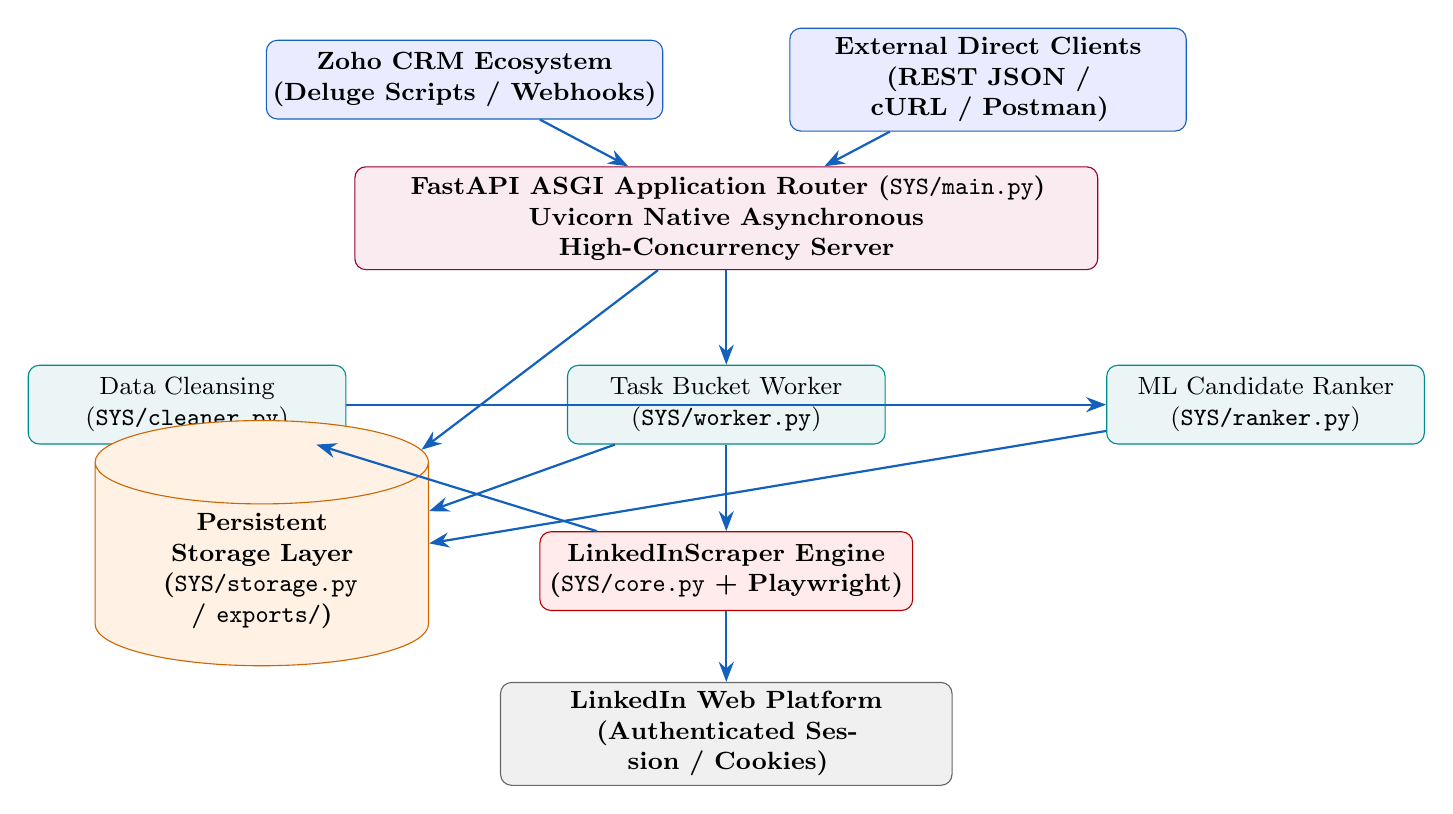
\begin{tikzpicture}[
    node distance=1.1cm and 1.2cm,
    every node/.style={font=\small, align=center},
    client/.style={rectangle, rounded corners=4pt, draw=primaryblue, fill=blue!8, text width=4.8cm, minimum height=1.0cm, font=\small\bfseries},
    router/.style={rectangle, rounded corners=4pt, draw=purple!80!black, fill=purple!8, text width=9.2cm, minimum height=1.1cm, font=\small\bfseries},
    subsys/.style={rectangle, rounded corners=4pt, draw=accentteal, fill=teal!8, text width=3.8cm, minimum height=1.0cm, font=\small},
    engine/.style={rectangle, rounded corners=4pt, draw=red!70!black, fill=red!8, text width=4.5cm, minimum height=1.0cm, font=\small\bfseries},
    storage/.style={cylinder, shape border rotate=90, draw=orange!80!black, fill=orange!10, text width=4.0cm, minimum height=1.1cm, aspect=0.25, font=\small\bfseries},
    target/.style={rectangle, rounded corners=4pt, draw=gray!80!black, fill=gray!12, text width=5.5cm, minimum height=1.0cm, font=\small\bfseries},
    arrow/.style={-{Stealth[scale=1.1]}, thick, draw=primaryblue}
]

% Clients
\node[client] (zoho) {Zoho CRM Ecosystem\\(Deluge Scripts / Webhooks)};
\node[client, right=1.6cm of zoho] (dev) {External Direct Clients\\(REST JSON / cURL / Postman)};

% FastAPI Router
\node[router, below=1.1cm of $(zoho)!0.5!(dev)$] (api) {FastAPI ASGI Application Router (\texttt{SYS/main.py})\\Uvicorn Native Asynchronous High-Concurrency Server};

% Core Subsystems
\node[subsys, below left=1.2cm and 0.1cm of api] (cleaner) {Data Cleansing\\(\texttt{SYS/cleaner.py})};
\node[subsys, below=1.2cm of api] (worker) {Task Bucket Worker\\(\texttt{SYS/worker.py})};
\node[subsys, below right=1.2cm and 0.1cm of api] (ranker) {ML Candidate Ranker\\(\texttt{SYS/ranker.py})};

% Scraping Engine
\node[engine, below=1.1cm of worker] (core) {LinkedInScraper Engine\\(\texttt{SYS/core.py} + Playwright)};

% Target Platform
\node[target, below=0.9cm of core] (linkedin) {LinkedIn Web Platform\\(Authenticated Session / Cookies)};

% Storage Subsystem
\node[storage, left=1.4cm of core] (storage) {Persistent Storage Layer\\(\texttt{SYS/storage.py} / \texttt{exports/})};

% Connections
\draw[arrow] (zoho) -- (api);
\draw[arrow] (dev) -- (api);
\draw[arrow] (api) -- (worker);
\draw[arrow] (api) -- (storage);
\draw[arrow] (worker) -- (core);
\draw[arrow] (core) -- (linkedin);
\draw[arrow] (core) -- (cleaner);
\draw[arrow] (cleaner) -- (ranker);
\draw[arrow] (ranker) -- (storage);
\draw[arrow] (worker) -- (storage);

\end{tikzpicture}
}
\end{tcolorbox}
\vspace{0.2cm}
\caption{Persona - Linkedin Scrapper platform Microservice Architecture \& Component Topology}
\label{fig:sys_topology}
\end{figure}
\clearpage

% -------------------------------------------------------------------------
% STANDALONE FULL-PAGE FIGURE 1.2
% -------------------------------------------------------------------------
\clearpage
\begin{figure}[p]
\centering
\begin{tcolorbox}[colback=white,colframe=purple!80!black,title=\textbf{Figure 1.2: Application Execution Lifecycle \& Event Loop Flow},width=\textwidth,arc=3mm]
\centering
\resizebox{0.90\textwidth}{!}{
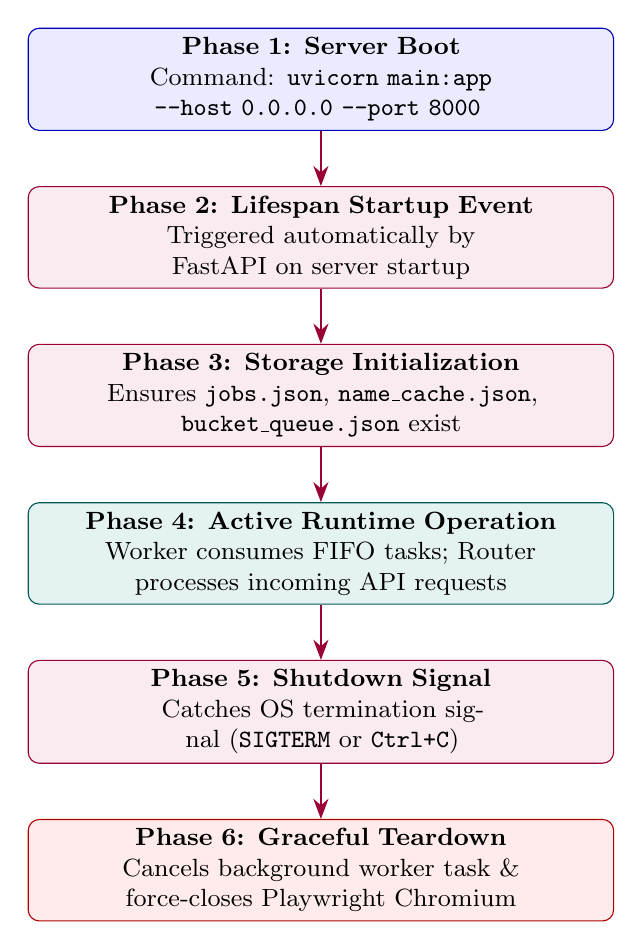
\begin{tikzpicture}[
    node distance=1.1cm and 1.5cm,
    box/.style={rectangle, rounded corners=4pt, draw=purple!80!black, fill=purple!8, text width=7.2cm, minimum height=1.0cm, align=center, font=\small},
    arrow/.style={-{Stealth[scale=1.1]}, thick, draw=purple!80!black}
]

\node[box, fill=blue!8, draw=blue!70!black] (boot) {\textbf{Phase 1: Server Boot}\\Command: \texttt{uvicorn main:app --host 0.0.0.0 --port 8000}};
\node[box, below=0.7cm of boot] (lifespan_start) {\textbf{Phase 2: Lifespan Startup Event}\\Triggered automatically by FastAPI on server startup};
\node[box, below=0.7cm of lifespan_start] (storage_init) {\textbf{Phase 3: Storage Initialization}\\Ensures \texttt{jobs.json}, \texttt{name\_cache.json}, \texttt{bucket\_queue.json} exist};
\node[box, below=0.7cm of storage_init, fill=teal!10, draw=teal!70!black] (worker_loop) {\textbf{Phase 4: Active Runtime Operation}\\Worker consumes FIFO tasks; Router processes incoming API requests};
\node[box, below=0.7cm of worker_loop] (shutdown_sig) {\textbf{Phase 5: Shutdown Signal}\\Catches OS termination signal (\texttt{SIGTERM} or \texttt{Ctrl+C})};
\node[box, below=0.7cm of shutdown_sig, fill=red!8, draw=red!70!black] (cleanup) {\textbf{Phase 6: Graceful Teardown}\\Cancels background worker task \& force-closes Playwright Chromium};

\draw[arrow] (boot) -- (lifespan_start);
\draw[arrow] (lifespan_start) -- (storage_init);
\draw[arrow] (storage_init) -- (worker_loop);
\draw[arrow] (worker_loop) -- (shutdown_sig);
\draw[arrow] (shutdown_sig) -- (cleanup);

\end{tikzpicture}
}
\end{tcolorbox}
\vspace{0.2cm}
\caption{FastAPI Application Lifespan Startup, Execution \& Shutdown Sequence}
\label{fig:lifespan_seq}
\end{figure}
\clearpage

% -------------------------------------------------------------------------
% CHAPTER 2: CROSS-PLATFORM INSTALLATION GUIDE
% -------------------------------------------------------------------------
\chapter{Cross-Platform Installation \& Setup Guide}

\section{System Requirements Matrix}
\begin{table}[h!]
\centering
\small
\begin{tabularx}{\textwidth}{l X X}
\toprule
\textbf{Component} & \textbf{Minimum Requirement} & \textbf{Recommended Production Requirement} \\
\midrule
Operating System & Windows 10/11, Ubuntu 20.04+, macOS 12+ & Ubuntu Linux 22.04 LTS (64-bit Server) \\
Python Version & Python 3.10.x & Python 3.11.x or 3.12.x \\
System Memory (RAM) & 2 GB RAM & 4 GB RAM or higher (Chromium page rendering) \\
Processor (CPU) & 1 Core & 2 vCPUs or higher \\
Disk Storage & 5 GB free disk space & 20 GB SSD storage \\
Network & Broadband connection & High-speed low-latency static IP / VPS \\
\bottomrule
\end{tabularx}
\caption{System Hardware and Software Prerequisites}
\label{tab:prereqs}
\end{table}

\section{Installation on Windows (Windows 10 / 11 / Server 2022)}
\begin{enumerate}[leftmargin=*]
    \item \textbf{Install Python 3.11+}: Download and install Python from \url{https://www.python.org/}. Ensure \textbf{``Add Python to PATH''} is checked during installation.
    \item \textbf{Open PowerShell as Administrator} and navigate to the project directory:
\begin{lstlisting}[language=bash]
cd D:\Projects\Int\Today_done\SYS
\end{lstlisting}
    \item \textbf{Create a Virtual Environment}:
\begin{lstlisting}[language=bash]
python -m venv venv
.\venv\Scripts\Activate.ps1
\end{lstlisting}
    \item \textbf{Install Dependencies \& Playwright Chromium}:
\begin{lstlisting}[language=bash]
pip install --upgrade pip
pip install -r requirements.txt
playwright install chromium
\end{lstlisting}
    \item \textbf{Configure Environment Variables}: Copy \texttt{.env.example} to \texttt{.env} and enter your LinkedIn credentials or \texttt{li\_at} cookie.
    \item \textbf{Launch the Application}: Run \texttt{start.bat} or launch directly:
\begin{lstlisting}[language=bash]
python -m uvicorn main:app --host 0.0.0.0 --port 8000 --reload
\end{lstlisting}
\end{enumerate}

\section{Installation on Linux (Ubuntu 22.04 LTS / Debian 12)}
\begin{enumerate}[leftmargin=*]
    \item \textbf{Update System Repositories and Install Prerequisites}:
\begin{lstlisting}[language=bash]
sudo apt update && sudo apt upgrade -y
sudo apt install -y python3-pip python3-venv git curl libglib2.0-0 libnss3 libnspr4
\end{lstlisting}
    \item \textbf{Setup Application Directory}:
\begin{lstlisting}[language=bash]
cd /opt/persona/SYS
python3 -m venv venv
source venv/bin/activate
\end{lstlisting}
    \item \textbf{Install Python Modules and Playwright System Libraries}:
\begin{lstlisting}[language=bash]
pip install --upgrade pip
pip install -r requirements.txt
playwright install chromium
playwright install-deps chromium
\end{lstlisting}
    \item \textbf{Configure Environment}:
\begin{lstlisting}[language=bash]
cp .env.example .env
nano .env
# Set HEADLESS=true, LINKEDIN_LI_AT=your_cookie
\end{lstlisting}
    \item \textbf{Launch with Production Script}:
\begin{lstlisting}[language=bash]
chmod +x start.sh
./start.sh
\end{lstlisting}
\end{enumerate}

\section{Installation on macOS (Apple Silicon M1/M2/M3 \& Intel)}
\begin{enumerate}[leftmargin=*]
    \item \textbf{Install Homebrew \& Python} (if not already installed):
\begin{lstlisting}[language=bash]
brew install python@3.11
\end{lstlisting}
    \item \textbf{Setup Virtual Environment}:
\begin{lstlisting}[language=bash]
cd /path/to/Today_done/SYS
python3 -m venv venv
source venv/bin/activate
\end{lstlisting}
    \item \textbf{Install Dependencies and Playwright}:
\begin{lstlisting}[language=bash]
pip install -r requirements.txt
playwright install chromium
\end{lstlisting}
    \item \textbf{Start Server}:
\begin{lstlisting}[language=bash]
uvicorn main:app --host 0.0.0.0 --port 8000 --reload
\end{lstlisting}
\end{enumerate}

\section{Production Cloud VPS Deployment (AWS, DigitalOcean, Hetzner, GCP)}
For production servers, configure a **Systemd Background Service** to ensure automatic startup and restart on crash:

\begin{lstlisting}[caption=Systemd Service Unit: /etc/systemd/system/persona.service]
[Unit]
Description=Persona - Linkedin Scrapper platform ASGI Microservice
After=network.target

[Service]
Type=simple
User=root
WorkingDirectory=/opt/persona/SYS
ExecStart=/opt/persona/SYS/venv/bin/uvicorn main:app --host 0.0.0.0 --port 8000 --workers 1
Restart=always
RestartSec=5
EnvironmentFile=/opt/persona/SYS/.env

[Install]
WantedBy=multi-user.target
\end{lstlisting}

Enable and start the service:
\begin{lstlisting}[language=bash]
sudo systemctl daemon-reload
sudo systemctl enable persona
sudo systemctl start persona
sudo systemctl status persona
\end{lstlisting}

% -------------------------------------------------------------------------
% CHAPTER 3: DATA CLEANSING & SANITIZATION PIPELINE
% -------------------------------------------------------------------------
\chapter{Data Cleansing \& Sanitization Pipeline}

\section{The LinkedIn DOM Noise Problem}
As detailed in Figure~\ref{fig:cleaner_pipeline}, modern single-page application (SPA) architectures on LinkedIn render dynamic navigation elements, footer links, language pickers, and interactive action buttons into the DOM tree. When scraping profile sections, standard DOM traversals accidentally capture UI garbage such as:
\begin{itemize}[leftmargin=*]
    \item Footer links: \textit{``Accessibility'', ``Talent Solutions'', ``Community Guidelines'', ``Privacy \& Terms''}.
    \item Language selector lists: \textit{``العربية (Arabic)'', ``Deutsch (German)'', ``English (English)'', ``Español (Spanish)''}.
    \item Button artifacts: \textit{``Show all 12 experiences'', ``See more'', ``...more'', ``Show credential'', ``500+ connections''}.
\end{itemize}

\section{The 7-Stage Cleansing Algorithm (\texttt{cleaner.py})}
To guarantee clean CRM records, \texttt{cleaner.py} subjects all scraped data to a 7-stage sanitization pipeline:
\begin{enumerate}[leftmargin=*]
    \item \textbf{Stage 1: Top-Level Value Cleaning (\texttt{\_clean\_value})}: Normalizes null-like representations (\texttt{"none"}, \texttt{"null"}, \texttt{"n/a"}, \texttt{""}) to clean Python \texttt{None} objects or stripped strings.
    \item \textbf{Stage 2: About Text Cleansing (\texttt{\_clean\_about})}: Scans text for footer cutoff markers (\texttt{"Accessibility\textbackslash nTalent Solutions"}), truncates trailing UI disclaimers, and strips trailing ellipsis markers (\texttt{"...more"}, \texttt{"see more"}).
    \item \textbf{Stage 3: Work Experience Sanitization (\texttt{\_clean\_experience\_list})}: Validates that both \texttt{title} and \texttt{company} contain valid text, eliminates UI button artifacts, and deduplicates identical job entries.
    \item \textbf{Stage 4: Education Credentials Sanitization (\texttt{\_clean\_education\_list})}: Validates school names and degree titles while discarding accidental skill tags.
    \item \textbf{Stage 5: Certifications Sanitization (\texttt{\_clean\_certification\_list})}: Removes \texttt{"Show credential"} and badge buttons, retaining issuing authority and certification names.
    \item \textbf{Stage 6: Real Language Validation (\texttt{\_clean\_languages\_list})}: Evaluates candidate languages against a strict allowlist (\texttt{\_REAL\_LANGUAGE\_NAMES}) to ensure language picker dropdowns are never recorded as candidate proficiencies.
    \item \textbf{Stage 7: Skills Deduplication (\texttt{\_clean\_skills\_list})}: Normalizes skills into standardized dictionaries, deduplicates case-insensitively, and filters out long project descriptions that leaked into skill tags.
\end{enumerate}

% -------------------------------------------------------------------------
% STANDALONE FULL-PAGE FIGURE 2.1
% -------------------------------------------------------------------------
\clearpage
\begin{figure}[p]
\centering
\begin{tcolorbox}[colback=white,colframe=accentteal,title=\textbf{Figure 2.1: 7-Stage Profile Data Cleansing \& Normalization Pipeline},width=\textwidth,arc=3mm]
\centering
\resizebox{0.88\textwidth}{!}{
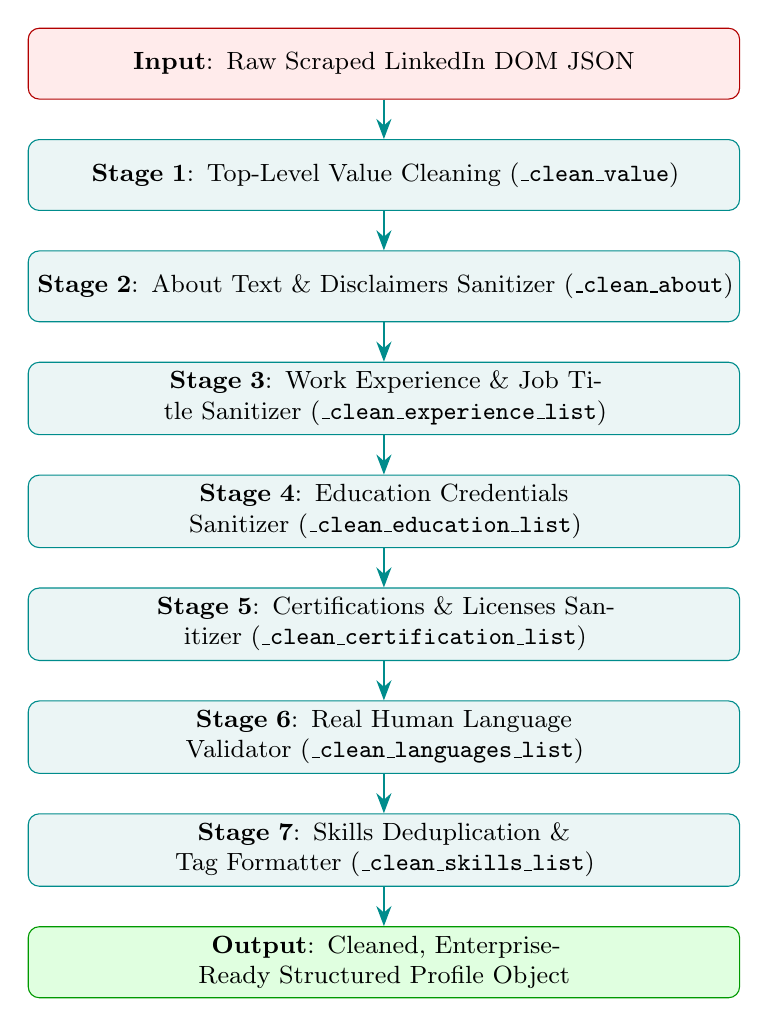
\begin{tikzpicture}[
    node distance=0.8cm and 1.2cm,
    stepnode/.style={rectangle, rounded corners=4pt, draw=accentteal, fill=teal!8, text width=8.8cm, minimum height=0.9cm, align=center, font=\small},
    arrow/.style={-{Stealth[scale=1.1]}, thick, draw=accentteal}
]

\node[stepnode, fill=red!8, draw=red!70!black] (raw) {\textbf{Input}: Raw Scraped LinkedIn DOM JSON};
\node[stepnode, below=0.5cm of raw] (s1) {\textbf{Stage 1}: Top-Level Value Cleaning (\texttt{\_clean\_value})};
\node[stepnode, below=0.5cm of s1] (s2) {\textbf{Stage 2}: About Text \& Disclaimers Sanitizer (\texttt{\_clean\_about})};
\node[stepnode, below=0.5cm of s2] (s3) {\textbf{Stage 3}: Work Experience \& Job Title Sanitizer (\texttt{\_clean\_experience\_list})};
\node[stepnode, below=0.5cm of s3] (s4) {\textbf{Stage 4}: Education Credentials Sanitizer (\texttt{\_clean\_education\_list})};
\node[stepnode, below=0.5cm of s4] (s5) {\textbf{Stage 5}: Certifications \& Licenses Sanitizer (\texttt{\_clean\_certification\_list})};
\node[stepnode, below=0.5cm of s5] (s6) {\textbf{Stage 6}: Real Human Language Validator (\texttt{\_clean\_languages\_list})};
\node[stepnode, below=0.5cm of s6] (s7) {\textbf{Stage 7}: Skills Deduplication \& Tag Formatter (\texttt{\_clean\_skills\_list})};
\node[stepnode, below=0.5cm of s7, fill=green!12, draw=green!60!black] (out) {\textbf{Output}: Cleaned, Enterprise-Ready Structured Profile Object};

\draw[arrow] (raw) -- (s1);
\draw[arrow] (s1) -- (s2);
\draw[arrow] (s2) -- (s3);
\draw[arrow] (s3) -- (s4);
\draw[arrow] (s4) -- (s5);
\draw[arrow] (s5) -- (s6);
\draw[arrow] (s6) -- (s7);
\draw[arrow] (s7) -- (out);

\end{tikzpicture}
}
\end{tcolorbox}
\vspace{0.2cm}
\caption{7-Stage Profile Data Cleansing \& Normalization Pipeline Flowchart}
\label{fig:cleaner_pipeline}
\end{figure}
\clearpage

% -------------------------------------------------------------------------
% CHAPTER 4: ML CANDIDATE SCORING & RANKING ENGINE
% -------------------------------------------------------------------------
\chapter{Machine Learning Candidate Scoring Model}

\section{Mathematical Formulation (\texttt{ranker.py})}
Persona incorporates a weighted candidate scoring model designed to score and rank candidates based on profile richness and domain alignment.

The total score $S_{\text{total}} \in [0, 150]$ is calculated as:
\begin{equation}
    S_{\text{total}} = S_{\text{completeness}} + S_{\text{field\_followers}}
\end{equation}

Where $S_{\text{completeness}} \in [0, 100]$ evaluates data completeness across 15 weighted features:
\begin{equation}
    S_{\text{completeness}} = \sum_{k=1}^{15} W_k \cdot f_k(\text{profile})
\end{equation}

\begin{table}[h!]
\centering
\small
\begin{tabularx}{\textwidth}{l c X}
\toprule
\textbf{Feature Metric ($k$)} & \textbf{Max Weight ($W_k$)} & \textbf{Evaluation Function ($f_k$)} \\
\midrule
\texttt{has\_headline} & 8 & $1$ if headline is present, $0$ otherwise \\
\texttt{headline\_length} & 4 & $\min(\text{length} / 120, 1.0)$ \\
\texttt{has\_about} & 8 & $1$ if about section is present, $0$ otherwise \\
\texttt{about\_length} & 6 & $\min(\text{length} / 800, 1.0)$ \\
\texttt{experience\_count} & 15 & $\min(N_{\text{exp}} \times 3, 15)$ \\
\texttt{experience\_quality} & 8 & Richness score based on description length ($>80$ chars) and dates \\
\texttt{education\_count} & 8 & $\min(N_{\text{edu}} \times 4, 8)$ \\
\texttt{skills\_count} & 10 & $\min(N_{\text{skills}} \times 1, 10)$ \\
\texttt{certifications} & 8 & $\min(N_{\text{certs}} \times 2, 8)$ \\
\texttt{featured} & 5 & $1$ if featured media/links exist, $0$ otherwise \\
\texttt{connections\_known} & 6 & Connection scaling: $\min(N_{\text{conn}} / 500, 1.0) \times 6$ \\
\texttt{profile\_photo} & 4 & Inferred avatar presence baseline \\
\texttt{recommendations} & 5 & $\min(N_{\text{recs}} \times 2.5, 5)$ \\
\texttt{volunteer} & 3 & $1$ if volunteer history exists, $0$ otherwise \\
\texttt{languages} & 2 & $\min(N_{\text{langs}} \times 1, 2)$ \\
\bottomrule
\end{tabularx}
\caption{Profile Completeness Evaluation Weight Matrix}
\label{tab:scoring_matrix}
\end{table}

\section{Field-Aligned Connection Density ($S_{\text{field\_followers}}$)}
The second term evaluates domain authority by matching candidate connection volumes against an 11-category domain taxonomy (Software \& IT, Data \& Analytics, Finance, Healthcare, Engineering, etc.):
\begin{equation}
    S_{\text{field\_followers}} = 50 \times \left( 0.6 \cdot \min\left(\frac{N_{\text{conn}}}{1000}, 1.0\right) + 0.4 \cdot \text{KeywordDensity}(\text{Category}) \right)
\end{equation}

\section{Classification Tiers}
\begin{itemize}[noitemsep, topsep=2pt]
    \item \textbf{Elite ($S_{\text{total}} \ge 120$)}: Industry leaders, senior architects, C-level executives.
    \item \textbf{Expert ($100 \le S_{\text{total}} < 120$)}: Senior professionals with comprehensive verified profiles.
    \item \textbf{Strong ($80 \le S_{\text{total}} < 100$)}: Mid-to-senior candidates with solid domain histories.
    \item \textbf{Moderate ($60 \le S_{\text{total}} < 80$)}: Early-career candidates or partially completed profiles.
    \item \textbf{Beginner ($S_{\text{total}} < 60$)}: Minimal profile presence or entry-level profiles.
\end{itemize}

% -------------------------------------------------------------------------
% CHAPTER 5: TASK BUCKET & BACKGROUND WORKER
% -------------------------------------------------------------------------
\chapter{Task Bucket Queue \& Background Worker Subsystem}

\section{Single-Worker Queue Invariant}
As shown in Figure~\ref{fig:bucket_state_machine}, LinkedIn strictly monitors concurrent requests from single user accounts. To eliminate the risk of automated account bans, Persona enforces a **Single-Worker FIFO Processing Invariant**:
\begin{enumerate}[leftmargin=*]
    \item All requests from Zoho CRM, bulk imports, and direct API calls are appended to the atomic queue file \texttt{bucket\_queue.json}.
    \item A single background coroutine consumer (\texttt{\_bucket\_worker\_loop}) runs continuously on the \texttt{asyncio} event loop.
    \item The worker pops exactly one pending task at a time, checks session authentication, executes the scrape, saves the result, and rests before the next task.
\end{enumerate}

\section{Anti-Ban Randomized Delay Algorithm}
To mimic natural human browsing behavior, the worker enforces a randomized jitter rest interval between consecutive scrape jobs:
\begin{equation}
    T_{\text{rest}} \sim \mathcal{U}(\max(10, B), \max(20, B + 15))
\end{equation}
Where $B$ is the configured base rest interval (default $30\text{ seconds}$).

% -------------------------------------------------------------------------
% STANDALONE FULL-PAGE FIGURE 3.1
% -------------------------------------------------------------------------
\clearpage
\begin{figure}[p]
\centering
\begin{tcolorbox}[colback=white,colframe=orange!80!black,title=\textbf{Figure 4.1: Task Bucket Queue State Machine \& Background Worker Cycle},width=\textwidth,arc=3mm]
\centering
\resizebox{0.88\textwidth}{!}{
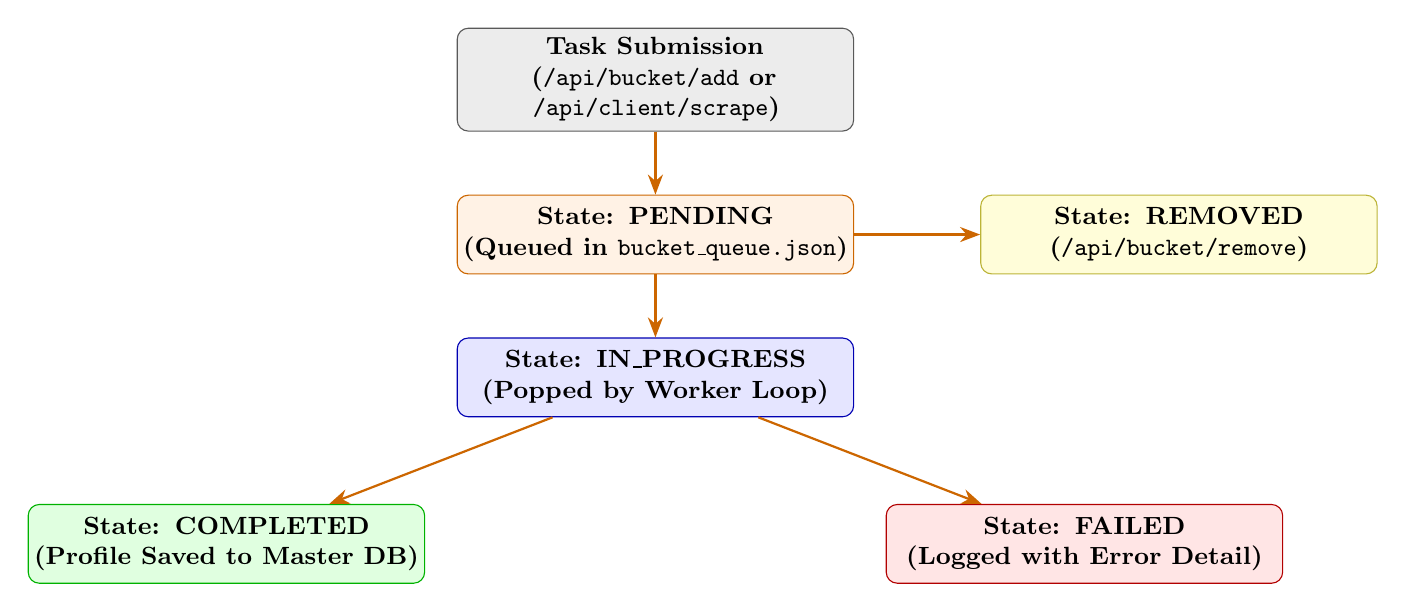
\begin{tikzpicture}[
    node distance=1.1cm and 1.5cm,
    statenode/.style={rectangle, rounded corners=4pt, draw=orange!80!black, fill=orange!10, text width=4.8cm, minimum height=1.0cm, align=center, font=\small\bfseries},
    arrow/.style={-{Stealth[scale=1.1]}, thick, draw=orange!80!black}
]

\node[statenode, fill=gray!15, draw=gray!70!black] (init) {Task Submission\\(\texttt{/api/bucket/add} or \texttt{/api/client/scrape})};
\node[statenode, below=0.8cm of init] (pending) {State: PENDING\\(Queued in \texttt{bucket\_queue.json})};
\node[statenode, below=0.8cm of pending, fill=blue!10, draw=blue!70!black] (inprogress) {State: IN\_PROGRESS\\(Popped by Worker Loop)};
\node[statenode, below left=1.1cm and 0.4cm of inprogress, fill=green!12, draw=green!70!black] (completed) {State: COMPLETED\\(Profile Saved to Master DB)};
\node[statenode, below right=1.1cm and 0.4cm of inprogress, fill=red!10, draw=red!70!black] (failed) {State: FAILED\\(Logged with Error Detail)};
\node[statenode, right=1.6cm of pending, fill=yellow!15, draw=yellow!70!black] (removed) {State: REMOVED\\(\texttt{/api/bucket/remove})};

\draw[arrow] (init) -- (pending);
\draw[arrow] (pending) -- (inprogress);
\draw[arrow] (pending) -- (removed);
\draw[arrow] (inprogress) -- (completed);
\draw[arrow] (inprogress) -- (failed);

\end{tikzpicture}
}
\end{tcolorbox}
\vspace{0.2cm}
\caption{Task Bucket Queue Processing State Machine}
\label{fig:bucket_state_machine}
\end{figure}
\clearpage

% -------------------------------------------------------------------------
% CHAPTER 6: COMPLETE REST API REFERENCE MANUAL
% -------------------------------------------------------------------------
\chapter{Complete REST API Reference Specification}

\section{Overview of All 34 REST Endpoints}
The Persona API exposes 34 routes categorized into 5 functional groups:

\subsection{1. Search \& Scrape Endpoints}

\subsubsection{\texttt{POST /api/client/scrape}}
\textbf{Primary endpoint for Zoho CRM candidate enrichment.}
\begin{itemize}[noitemsep]
    \item \textbf{Method}: \texttt{POST}
    \item \textbf{Status Codes}: \texttt{200 OK} (cached), \texttt{202 Accepted} (queued), \texttt{400 Bad Request}.
    \item \textbf{Request Body Schema}:
\end{itemize}
\begin{lstlisting}[language=json]
{
  "name": "Bawantha Beliwaththa",
  "profile_url": "https://www.linkedin.com/in/bawantha-beliwaththa"
}
\end{lstlisting}
\begin{itemize}[noitemsep]
    \item \textbf{Response (202 Accepted - Queued)}:
\end{itemize}
\begin{lstlisting}[language=json]
{
  "success": true,
  "status": "queued",
  "reference_number": "f97133ad-0f4c-4782-808f-3b72288cb6a8",
  "message": "Task queued in the bucket. The worker will process it automatically."
}
\end{lstlisting}

\subsubsection{\texttt{POST /api/scraper/search}}
Direct search for candidate profiles by structured criteria.
\begin{lstlisting}[language=json]
// Request:
{
  "first_name": "Hansika",
  "last_name": "Kavindi",
  "company": "Virtusa",
  "max_results": 5
}
\end{lstlisting}

\subsubsection{\texttt{POST /api/scraper/search-and-extract}}
Searches for top matches and extracts their full profiles immediately.

\subsubsection{\texttt{POST /api/scraper/search-contact-info}}
Extracts emails, phone numbers, and portfolio websites from candidate profile URLs.

\subsection{2. Track \& Status Retrieval Endpoints}

\subsubsection{\texttt{GET /api/client/scrape-status}}
\textbf{Case-insensitive status polling endpoint.}
\begin{itemize}[noitemsep]
    \item \textbf{Parameters}: \texttt{task\_id} (UUID) or \texttt{name} (string).
    \item \textbf{Response (202 Accepted - In Progress)}:
\end{itemize}
\begin{lstlisting}[language=json]
{
  "success": true,
  "status": "in_progress",
  "queue_position": 1,
  "queue_total": 4,
  "message": "Currently scraping LinkedIn profile..."
}
\end{lstlisting}
\begin{itemize}[noitemsep]
    \item \textbf{Response (200 OK - Completed)}:
\end{itemize}
\begin{lstlisting}[language=json]
{
  "success": true,
  "status": "completed",
  "profiles": [
    {
      "name": "Navod Ranasinghe",
      "headline": "Senior Data Engineer",
      "location": "Colombo, Sri Lanka",
      "profile_url": "https://www.linkedin.com/in/navod-ranasinghe",
      "current_job": { "title": "Senior Data Engineer", "company": "TechCorp" },
      "experience": [ ... ],
      "education": [ ... ],
      "skills": [ {"skill": "Python"}, {"skill": "Apache Spark"} ]
    }
  ],
  "total": 1
}
\end{lstlisting}

\subsubsection{\texttt{GET/POST /api/client/lookup-by-reference}}
Retrieves profile data by reference number or return code.

\subsubsection{\texttt{GET/POST /api/client/retrieve}}
Retrieves single job results by \texttt{return\_code}.

\subsubsection{\texttt{GET /api/scraper/stats}}
Returns scraper session authentication state and queue status.

\subsection{3. Bulk Search \& Batch Retrieval Endpoints}

\subsubsection{\texttt{POST /api/persona/bulk-scrape} (Alias: \texttt{POST /api/bulk/scrape})}
Enqueues multiple candidate profile URLs or names linked to a single batch \texttt{return\_code}.
\begin{lstlisting}[language=json]
{
  "profile_urls": [
    "https://www.linkedin.com/in/candidate-alpha",
    "https://www.linkedin.com/in/candidate-beta",
    "Yuvindu Lakshin Arthanayaka"
  ],
  "return_code": "BATCH-2026-08-001"
}
\end{lstlisting}

\subsubsection{\texttt{GET/POST /api/persona/bulk-retrieve} (Alias: \texttt{GET/POST /api/bulk/retrieve})}
Retrieves the consolidated array of scraped profiles once all batch tasks complete.

\subsubsection{\texttt{GET /api/client/download/csv} \& \texttt{GET /api/client/download/json}}
Direct file streaming downloads for individual or bulk scrape exports.

\subsection{4. Task Bucket / Basket Management Endpoints}

\subsubsection{\texttt{POST /api/bucket/add}}
Adds one or more queries or URLs into the Task Bucket queue.

\subsubsection{\texttt{POST /api/bucket/add-search}}
Adds a structured person search query into the Task Bucket.

\subsubsection{\texttt{POST /api/bucket/upload}}
Accepts \texttt{multipart/form-data} file uploads (\texttt{.csv} or \texttt{.json}) containing hundreds of lead rows.

\subsubsection{\texttt{GET /api/bucket/status}}
Returns full queue health: \texttt{pending}, \texttt{in\_progress}, \texttt{completed}, and \texttt{failed} counts.

\subsubsection{\texttt{POST /api/bucket/pause} \& \texttt{POST /api/bucket/resume}}
Pauses and resumes the background queue consumer.

\subsubsection{\texttt{POST /api/bucket/clear} \& \texttt{POST /api/bucket/remove}}
Cleans up completed/failed records or removes a specific pending task by ID.

\subsubsection{\texttt{POST /api/bucket/config}}
Configures rest interval between tasks: \texttt{\{"rest\_seconds": 30\}}.

\subsection{5. Scraper Session \& Authentication Endpoints}
\begin{itemize}[noitemsep, topsep=2pt]
    \item \texttt{POST /api/scraper/init}: Initializes Chromium instance (\texttt{headless=true/false}).
    \item \texttt{POST /api/scraper/login}: Form-based authentication with email and password.
    \item \texttt{POST /api/scraper/login-cookie}: Cookie-based instant login with \texttt{li\_at}.
    \item \texttt{POST /api/scraper/submit-pin}: Submits 2FA checkpoint PIN code.
    \item \texttt{POST /api/scraper/kill-browser}: Force-terminates orphaned Chromium browser instances.
\end{itemize}

% -------------------------------------------------------------------------
% CHAPTER 7: ZOHO CRM DELUGE INTEGRATION MANUAL
% -------------------------------------------------------------------------
\chapter{Zoho CRM Deluge Integration Manual}

\section{Two-Step Asynchronous Integration Architecture}
As illustrated in Figure~\ref{fig:zoho_seq}, because web scraping takes between $10$ to $30$ seconds per candidate, Zoho CRM workflows must not use blocking synchronous requests. The recommended pattern is:
\begin{enumerate}[leftmargin=*]
    \item \textbf{Step 1 (Trigger)}: When a user clicks ``Enrich Candidate'' in Zoho CRM, a Deluge script calls \texttt{POST /api/client/scrape}. Persona returns a tracking UUID reference immediately. The candidate record is marked \texttt{Enrichment\_Status = "In Progress"}.
    \item \textbf{Step 2 (Sync)}: A Zoho Scheduled Function runs periodically (every 5 minutes), calls \texttt{GET /api/client/scrape-status}, and automatically populates the candidate's fields upon completion.
\end{enumerate}

\section{Production Deluge Script: Trigger Enrichment}
\begin{lstlisting}[language=Java,caption=Zoho Deluge Candidate Trigger Script]
// Attach to: Zoho CRM -> Candidates Module -> Custom Button
candidateId = targetCandidateId.toLong();
candidateRecord = zoho.crm.getRecordById("Candidates", candidateId);

candidateName = candidateRecord.get("Full_Name");
linkedinUrl = candidateRecord.get("LinkedIn_URL");

serverUrl = "http://your-vps-ip:8000/api/client/scrape";

payload = Map();
if (linkedinUrl != null && linkedinUrl != "") {
    payload.put("profile_url", linkedinUrl);
} else {
    payload.put("name", candidateName);
}

headers = Map();
headers.put("Content-Type", "application/json");

response = invokeurl [
    url: serverUrl,
    type: POST,
    parameters: payload.toString(),
    headers: headers
];

if (response.get("success") == true) {
    if (response.get("cached") == true) {
        profiles = response.get("profiles");
        p = profiles.get(0);
        
        updateMap = Map();
        updateMap.put("Enrichment_Status", "Completed");
        updateMap.put("Current_Job", p.get("headline"));
        updateMap.put("Location", p.get("location"));
        updateMap.put("Summary", p.get("about"));
        zoho.crm.updateRecord("Candidates", candidateId, updateMap);
        return "Candidate enriched instantly from cache!";
    } else {
        refNumber = response.get("reference_number");
        updateMap = Map();
        updateMap.put("Enrichment_Status", "In Progress");
        updateMap.put("Persona_Reference", refNumber);
        zoho.crm.updateRecord("Candidates", candidateId, updateMap);
        return "Task queued in Persona bucket. Ref: " + refNumber;
    }
} else {
    return "Error: " + response.get("error");
}
\end{lstlisting}

\section{Production Deluge Script: Scheduled Polling Function}
\begin{lstlisting}[language=Java,caption=Zoho Deluge Scheduled Polling Sync Script]
// Configure in Zoho CRM -> Settings -> Functions -> Scheduled Function
inProgressCandidates = zoho.crm.searchRecords("Candidates", "(Enrichment_Status:equals:In Progress)");

for each candidate in inProgressCandidates {
    candidateId = candidate.get("id");
    refNumber = candidate.get("Persona_Reference");
    
    if (refNumber != null && refNumber != "") {
        statusUrl = "http://your-vps-ip:8000/api/client/scrape-status?task_id=" + refNumber;
        
        statusResponse = invokeurl [
            url: statusUrl,
            type: GET
        ];
        
        if (statusResponse.get("status") == "completed") {
            profiles = statusResponse.get("profiles");
            if (profiles.size() > 0) {
                p = profiles.get(0);
                
                updateData = Map();
                updateData.put("Enrichment_Status", "Completed");
                updateData.put("Current_Job", p.get("headline"));
                updateData.put("Location", p.get("location"));
                updateData.put("Summary", p.get("about"));
                updateData.put("LinkedIn_URL", p.get("profile_url"));
                
                skillsList = p.get("skills");
                skillsStr = "";
                for each s in skillsList {
                    skillsStr = skillsStr + s.get("skill") + ", ";
                }
                updateData.put("Key_Skills", skillsStr);
                
                zoho.crm.updateRecord("Candidates", candidateId, updateData);
                info "Enriched Candidate ID: " + candidateId;
            }
        } else if (statusResponse.get("status") == "failed") {
            errData = Map();
            errData.put("Enrichment_Status", "Failed");
            errData.put("Enrichment_Error", statusResponse.get("error"));
            zoho.crm.updateRecord("Candidates", candidateId, errData);
        }
    }
}
\end{lstlisting}

% -------------------------------------------------------------------------
% STANDALONE FULL-PAGE FIGURE 6.1
% -------------------------------------------------------------------------
\clearpage
\begin{figure}[p]
\centering
\begin{tcolorbox}[colback=white,colframe=primaryblue,title=\textbf{Figure 5.1: Zoho CRM Asynchronous Webhook \& Polling Sequence Flow},width=\textwidth,arc=3mm]
\centering
\resizebox{0.90\textwidth}{!}{
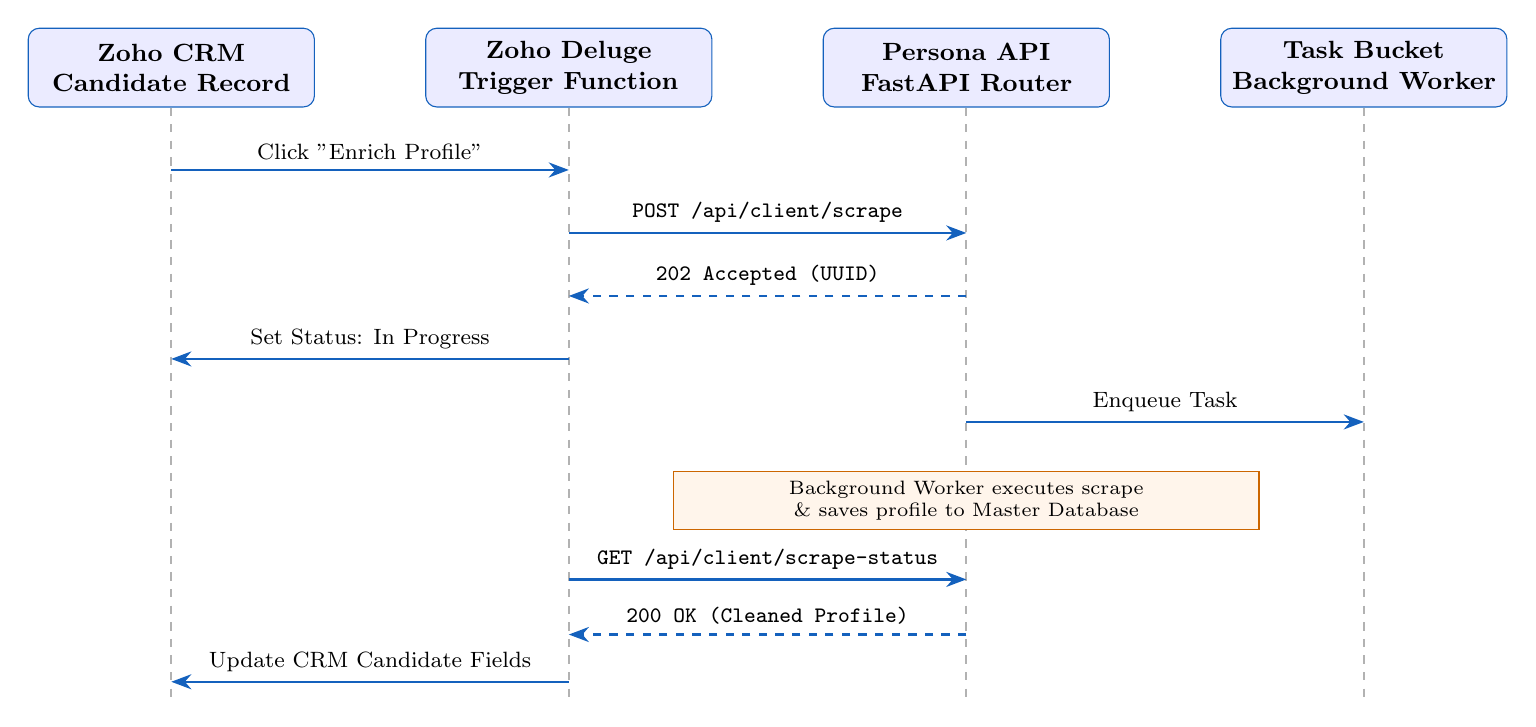
\begin{tikzpicture}[
    node distance=1.2cm and 2.2cm,
    actor/.style={rectangle, rounded corners=4pt, draw=primaryblue, fill=blue!8, text width=3.4cm, minimum height=1.0cm, align=center, font=\small\bfseries},
    lifeline/.style={thick, dashed, draw=gray!60},
    msg/.style={-{Stealth[scale=1.1]}, thick, draw=primaryblue, font=\footnotesize},
    reply/.style={-{Stealth[scale=1.1]}, thick, dashed, draw=primaryblue, font=\footnotesize}
]

% Actors
\node[actor] (crm) {Zoho CRM\\Candidate Record};
\node[actor, right=1.4cm of crm] (deluge) {Zoho Deluge\\Trigger Function};
\node[actor, right=1.4cm of deluge] (api) {Persona API\\FastAPI Router};
\node[actor, right=1.4cm of api] (worker) {Task Bucket\\Background Worker};

% Lifelines
\draw[lifeline] (crm) -- ++(0,-8.0);
\draw[lifeline] (deluge) -- ++(0,-8.0);
\draw[lifeline] (api) -- ++(0,-8.0);
\draw[lifeline] (worker) -- ++(0,-8.0);

% Messages
\draw[msg] ($(crm)+(0,-1.3)$) -- node[above]{Click "Enrich Profile"} ($(deluge)+(0,-1.3)$);
\draw[msg] ($(deluge)+(0,-2.1)$) -- node[above]{\texttt{POST /api/client/scrape}} ($(api)+(0,-2.1)$);
\draw[reply] ($(api)+(0,-2.9)$) -- node[above]{\texttt{202 Accepted (UUID)}} ($(deluge)+(0,-2.9)$);
\draw[msg] ($(deluge)+(0,-3.7)$) -- node[above]{Set Status: In Progress} ($(crm)+(0,-3.7)$);
\draw[msg] ($(api)+(0,-4.5)$) -- node[above]{Enqueue Task} ($(worker)+(0,-4.5)$);

\node[draw=orange!80!black, fill=orange!8, text width=7.2cm, align=center, font=\scriptsize] at ($(api)+(0,-5.5)$) {Background Worker executes scrape \& saves profile to Master Database};

\draw[msg] ($(deluge)+(0,-6.5)$) -- node[above]{\texttt{GET /api/client/scrape-status}} ($(api)+(0,-6.5)$);
\draw[reply] ($(api)+(0,-7.2)$) -- node[above]{\texttt{200 OK (Cleaned Profile)}} ($(deluge)+(0,-7.2)$);
\draw[msg] ($(deluge)+(0,-7.8)$) -- node[above]{Update CRM Candidate Fields} ($(crm)+(0,-7.8)$);

\end{tikzpicture}
}
\end{tcolorbox}
\vspace{0.2cm}
\caption{Zoho CRM Asynchronous Webhook \& Polling Sequence Flow}
\label{fig:zoho_seq}
\end{figure}
\clearpage

% -------------------------------------------------------------------------
% CHAPTER 8: SOURCE CODE CATALOG
% -------------------------------------------------------------------------
\chapter{Source Code Reference \& Function Catalog}

\section{\texttt{main.py} Function Catalog}
\begin{itemize}[leftmargin=*]
    \item \texttt{lifespan(app)}: Asynchronous lifespan context manager that guarantees worker launch on startup and clean cancellation on shutdown.
    \item \texttt{client\_scrape(req)}: Primary Zoho route; evaluates name cache and dispatches to Task Bucket.
    \item \texttt{client\_scrape\_status(task\_id, name)}: Case-insensitive polling endpoint.
    \item \texttt{bulk\_scrape(req)}: Enqueues batch scrape items linked to a parent \texttt{return\_code}.
    \item \texttt{bulk\_retrieve(return\_code)}: Assembles consolidated profile lists for batch jobs.
    \item \texttt{bucket\_add(req)} / \texttt{bucket\_upload(file)}: Enqueues queries or parsed CSV/JSON files.
    \item \texttt{bucket\_pause()} / \texttt{bucket\_resume()} / \texttt{bucket\_clear()}: Worker execution controllers.
\end{itemize}

\section{\texttt{core.py} (\texttt{LinkedInScraper}) Function Catalog}
\begin{itemize}[leftmargin=*]
    \item \texttt{initialize()}: Spawns Playwright Chromium process with persistent user data directory and stealth arguments.
    \item \texttt{login(email, password)}: Handles form authentication and challenge detection.
    \item \texttt{login\_with\_cookie(li\_at)}: Injects session cookies for 2FA bypass.
    \item \texttt{search\_people(first\_name, last\_name, company, max\_results)}: Executes structured search queries on LinkedIn.
    \item \texttt{extract\_profile(profile\_url)}: Performs DOM extraction across experiences, education, skills, about, licenses, and languages.
    \item \texttt{extract\_contact\_info(profile\_url)}: Interacts with contact info overlay modals.
    \item \texttt{\_kill\_orphan\_chromium(marker)}: Cross-platform process terminator.
\end{itemize}

\section{\texttt{cleaner.py} Function Catalog}
\begin{itemize}[leftmargin=*]
    \item \texttt{sanitize\_profile(profile)}: High-level entrypoint running all 7 sanitization stages.
    \item \texttt{\_clean\_about(text)}: Purges footer lines and ellipsis artifacts.
    \item \texttt{\_clean\_experience\_list(list)}: Deduplicates jobs, validates titles and organizations.
    \item \texttt{\_clean\_education\_list(list)}: Normalizes degrees and institutions.
    \item \texttt{\_clean\_languages\_list(list)}: Filters out navigation language pickers.
    \item \texttt{\_clean\_skills\_list(list)}: Normalizes and deduplicates skills.
    \item \texttt{format\_experience\_for\_csv()} / \texttt{format\_education\_for\_csv()}: CSV serialization string helpers.
\end{itemize}

% -------------------------------------------------------------------------
% CHAPTER 9: DIAGNOSTICS & TROUBLESHOOTING
% -------------------------------------------------------------------------
\chapter{Diagnostics, Troubleshooting \& Recovery}

\begin{table}[h!]
\centering
\small
\begin{tabularx}{\textwidth}{l X X}
\toprule
\textbf{Observed Issue} & \textbf{Root Cause} & \textbf{Standard Recovery Protocol} \\
\midrule
\texttt{Browser context closed} & Chromium crashed due to memory limit & Worker auto-catches error, calls \texttt{\_kill\_orphan\_chromium()}, and starts fresh context on next item. \\
\texttt{Unauthenticated session} & LinkedIn cookie expired & Update \texttt{LINKEDIN\_LI\_AT} in \texttt{.env} or call \texttt{POST /api/scraper/login-cookie}. \\
\texttt{Lock file error on launch} & Lingering process holding lock & Call \texttt{POST /api/scraper/kill-browser} or execute \texttt{pkill -f chromium}. \\
\texttt{Zoho InvokeURL Timeout} & Synchronous blocking request in Zoho & Switch Zoho integration to the asynchronous two-step polling pattern. \\
\bottomrule
\end{tabularx}
\caption{Production Troubleshooting Matrix}
\label{tab:troubleshooting}
\end{table}

\vfill
\centering
\rule{\textwidth}{1pt}\\[0.3cm]
\textbf{PERSONA - LINKEDIN SCRAPPER PLATFORM}\\
\textbf{Engineered by Team Persona (2026)}

\end{document}
